%%%%%%%%%%%%%%%%%%
% Chapitre 1 - Les engrenages %
%%%%%%%%%%%%%%%%%%

\chapter{Les engrenages}

\section{Introduction}
	\noindent Les engrenages sont des pièces mécaniques qui permettent de transmettre du mouvement.ils sont surtout utilisés pour jouer sur les vitesses de rotation : on les réduit ou on les multiplie (plus rare). Elles sont réalisées à l'aide d'une fraiseuse et non par coulage de fer en raison de la géométrie de la pièce et de la précision nécessaire. La théorie qui sera présentée permet une facilité de fabrication et une bonne durée de vie.
	
\section{Historique}
	\begin{wrapfigure}[4]{l}{3.2cm}
	\vspace{-5mm}
	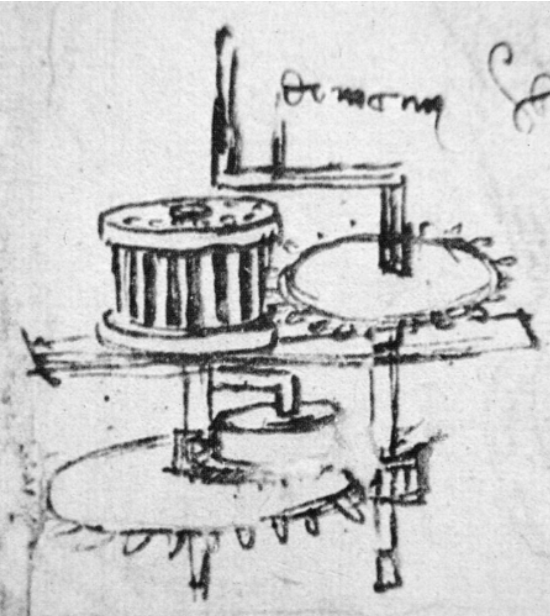
\includegraphics[scale=0.32]{ch1/1}
	\end{wrapfigure}
	\noindent Les premiers dessins effectués par Léonard de Vinci (15\up{ème} siècle n'étaient pas très clairs, mais on peut apercevoir, sur la figure de gauche, des dentures qui ressemble à celles utilisées aujourd'hui. \\\\\\\\\\\
	
	\begin{wrapfigure}[10]{r}{4.6cm}
	\vspace{-5mm}
	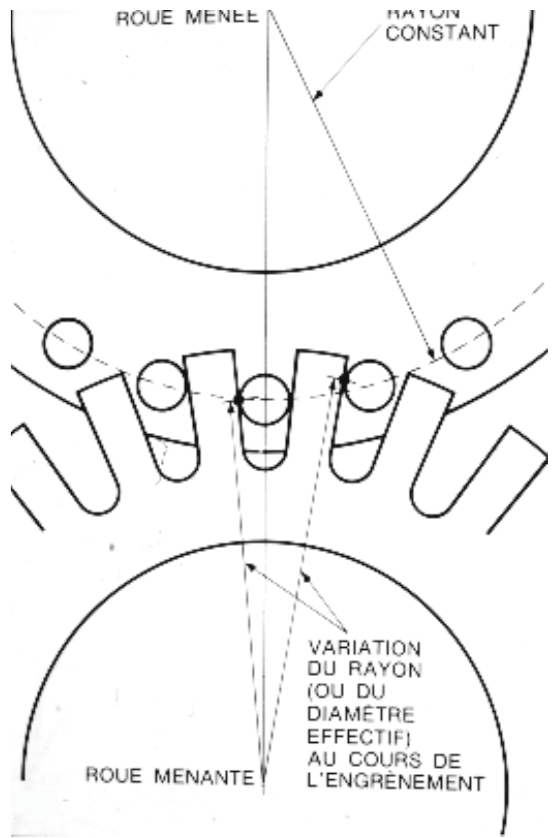
\includegraphics[scale=0.35]{ch1/2}
	\end{wrapfigure}	
	\noindent Un zoom sur ces fameux modèles permet d'avoir une vue plus moderne. Le problème de ce principe est que la transmission ne se fait pas de manière \textbf{homocinétique} (vitesse de sortie pas constante). La cause est que le point de contact entre la roue menée et la roue menante ne se trouve pas à la même distance (rayon d'entraînement) du centre de la roue menante durant la rotation.  \\
	Un second problème est le glissement important qui dégrade le matériel assez rapidement. Ce modèle n'est donc satisfaisant que pour de faibles vitesses et des puissances peu importantes. \\\\
	
	\begin{wrapfigure}[4]{l}{4.7cm}
	\vspace{-5mm}
	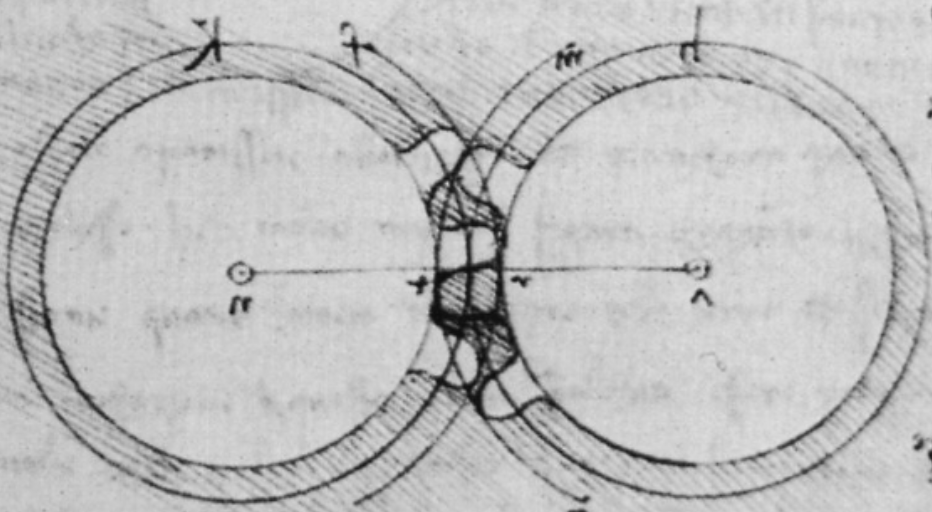
\includegraphics[scale=0.28]{ch1/3}
	\end{wrapfigure}	
	\noindent Ce dessin de de Vinci témoigne qu'on a cherché à créer une denture qui permettrait de limiter au mieux les deux problèmes majeurs énoncés. \\\\
	
	\begin{wrapfigure}[9]{r}{4cm}
	\vspace{-5mm}
	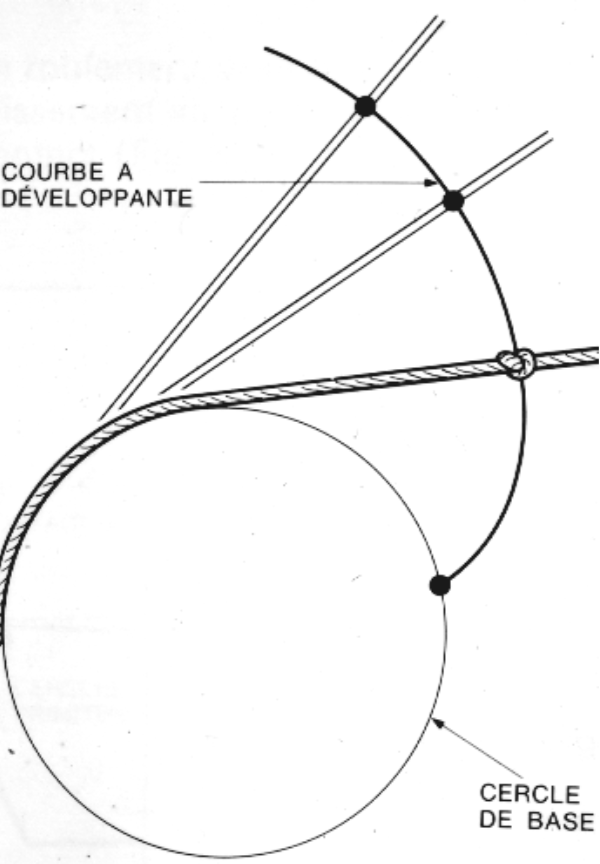
\includegraphics[scale=0.3]{ch1/4}
	\end{wrapfigure}	
	\noindent La solution adoptée par de Vinci a été de confectionner des dentures en \textbf{développante de cercle}. Il s'agit de la courbe obtenue lorsqu'on "déballe" un fil attaché par une extrémité à un cercle et préalablement accolé à celui-ci. Parmi d'autres théories, celle-ci à l'avantage de pouvoir être mise facilement sous équation et est donc programmable. En plus d'être facile, simple et bon marché, elle permet une \textbf{normalisation facile} afin qu'on ne doive pas faire fabriquer d'engrenages spécifiques. 
	
\section{Généralités}
	\begin{wrapfigure}[8]{l}{5.6cm}
	\vspace{-5mm}
	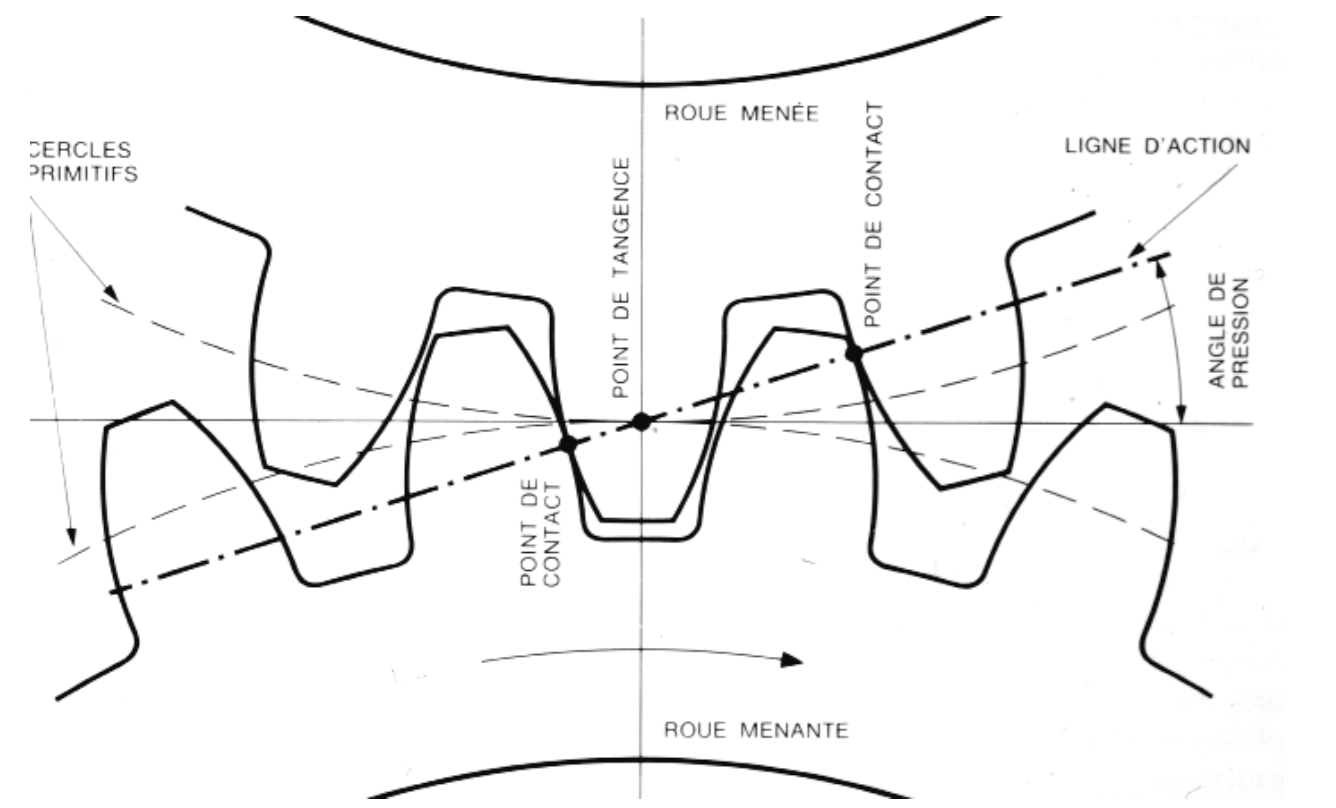
\includegraphics[scale=0.25]{ch1/5}
	\end{wrapfigure}	
	\noindent Une vue plus complexe nous permet, premièrement, de remarquer que dès le contact de deux nouvelles dents, deux autres rompent leur contact. Deuxièmement, il est possible de tracer deux cercles non tangents sauf en un seul point situé sur normale qui est le \textbf{point de tangence}. Dernièrement, l'évolution du point de contact en fonction du temps décrit une droite, la \textbf{ligne d'action} qui est toujours normale à la surface des dents au point de contact. La force de contact est donc toujours normale à cette surface également. La pente de cette droite est l'\textbf{angle de pression}. Pour transmettre une plus grande force, on a tendance à prendre un grand-angle de pression. \\
	
	\begin{wrapfigure}[5]{r}{5.6cm}
	\vspace{-5mm}
	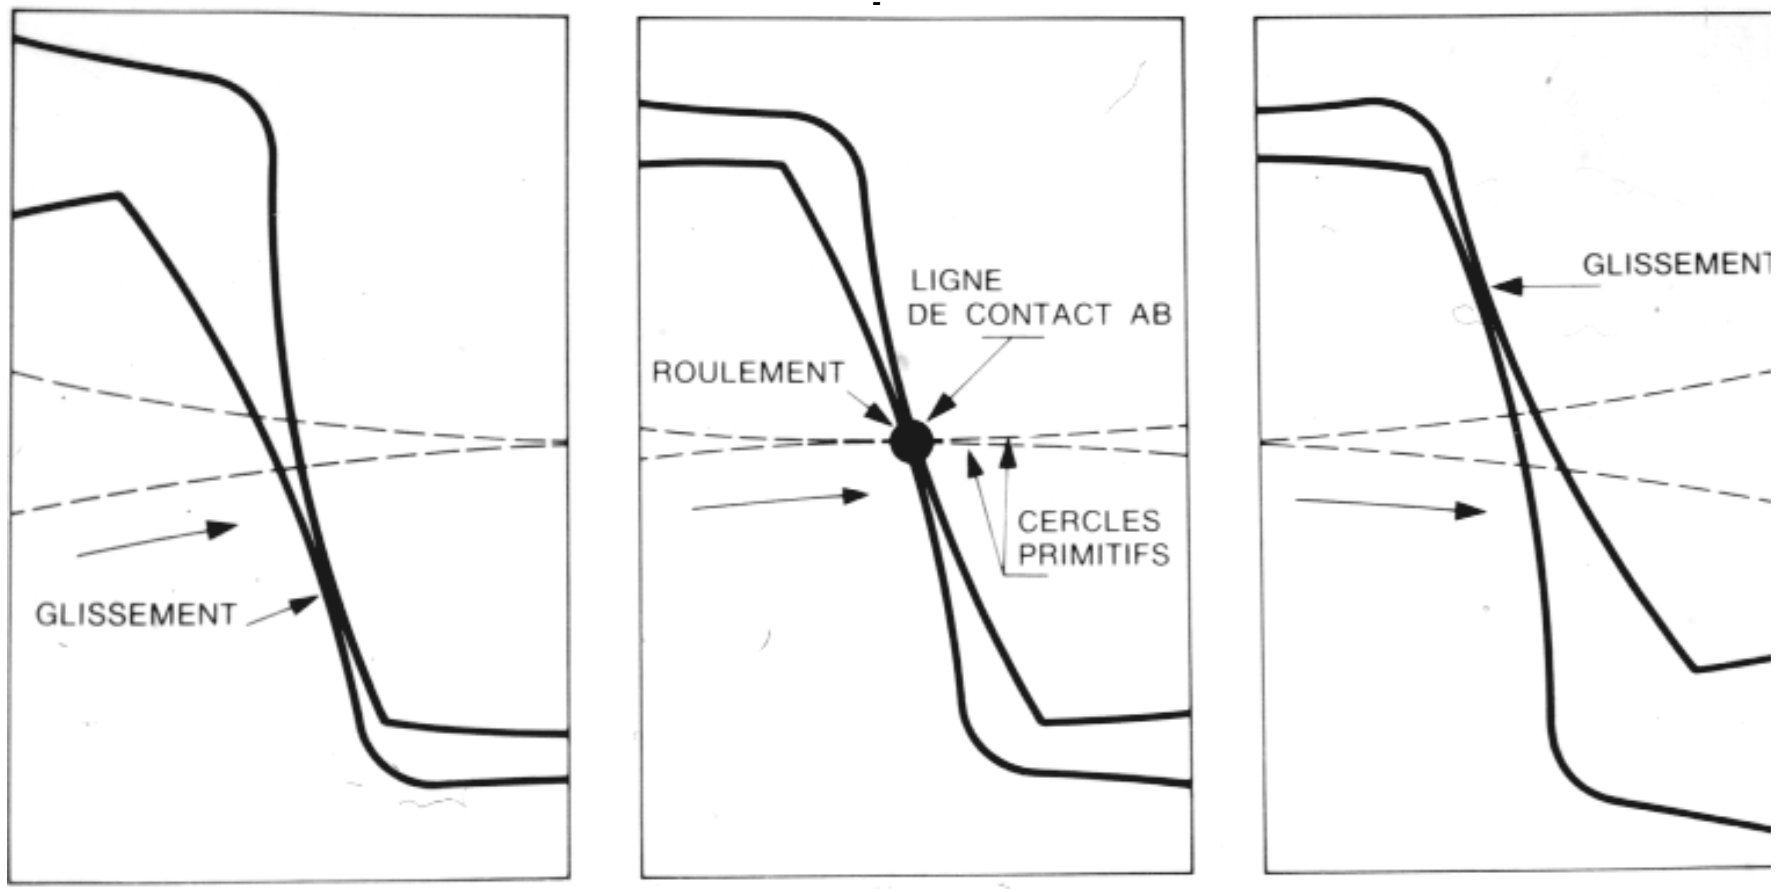
\includegraphics[scale=0.2]{ch1/6}
	\end{wrapfigure}	
	\noindent Néanmoins, on ne sait pas éviter les glissements. L'\textbf{engrènement} se déroule en 3 phases : une phase de glissement suivie du roulement au niveau du point de contact et une fin avec un nouveau glissement. 

\section{Différents types}
\subsection{Engrenages cylindriques à denture droite}
	\begin{wrapfigure}[5]{l}{2.5cm}
	\vspace{-5mm}
	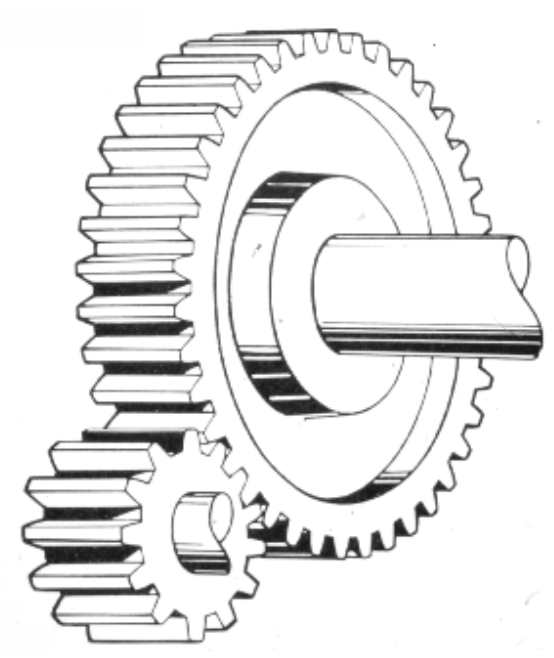
\includegraphics[scale=0.23]{ch1/7}
	\end{wrapfigure}	
	\noindent Ce modèle d'engrenage est de loin le plus courant. \textbf{Cylindrique} car l'engrenage possède une épaisseur, donnant une longueur aux dents. \textbf{A denture droite} car les dents sont disposées sur les génératrices de ce cylindre. Nous ne nous sommes pas attardés sur les principaux éléments de définition mais citons que l'angle de pression est de $20\degres$. \\
	
	\begin{wrapfigure}[5]{r}{2.5cm}
	\vspace{-5mm}
	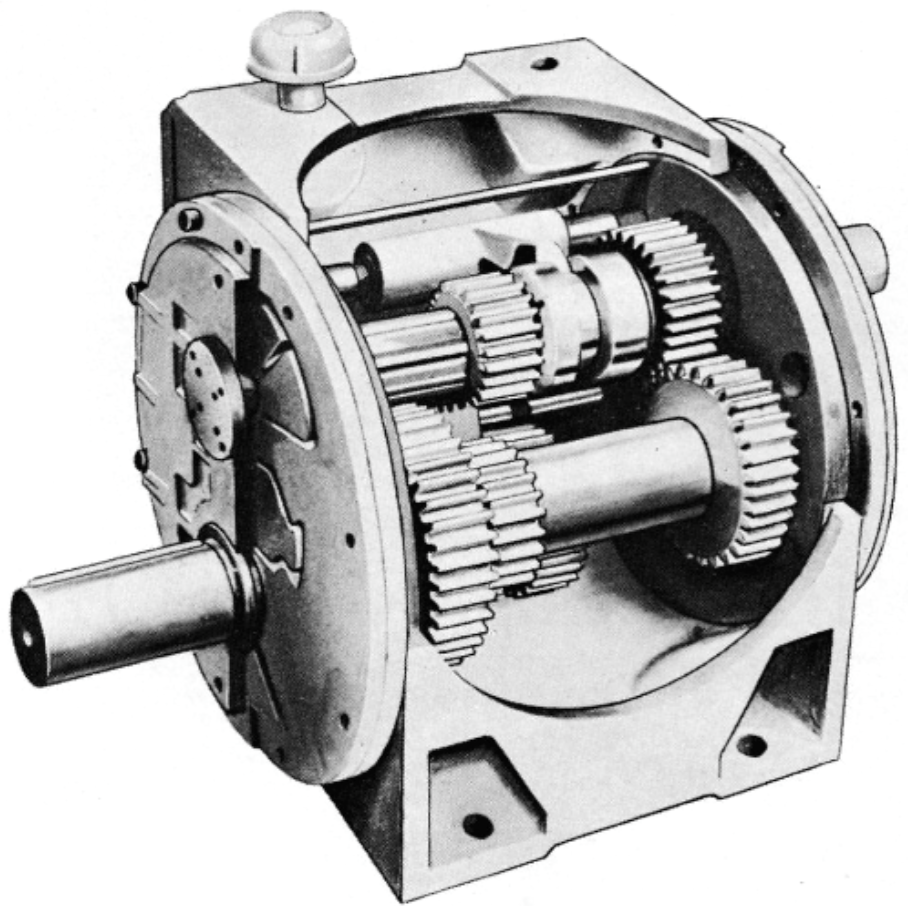
\includegraphics[scale=0.21]{ch1/8}
	\end{wrapfigure}	
	\noindent On peut bien sûr faire des combinaisons et former des boites d'engrenages. Cependant, ce type d'engrenage, dû à la largeur de la dent, présente l'inconvénient de faire durer le contact assez longtemps. Ceci provoque une flexion des dents et provoque du bruit.
	
\subsection{Contact et sens de rotation}
	\begin{itemize}
	\item Contact extérieur : sens inverse.
	\item Contact intérieur : même sens.
	\item Pignon crémaillère : transformation de rotation en translation ou inversément. 
	\end{itemize}
	
\subsection{Engrenages cylindriques à denture helicoïdale}
	\begin{wrapfigure}[5]{l}{2cm}
	\vspace{-5mm}
	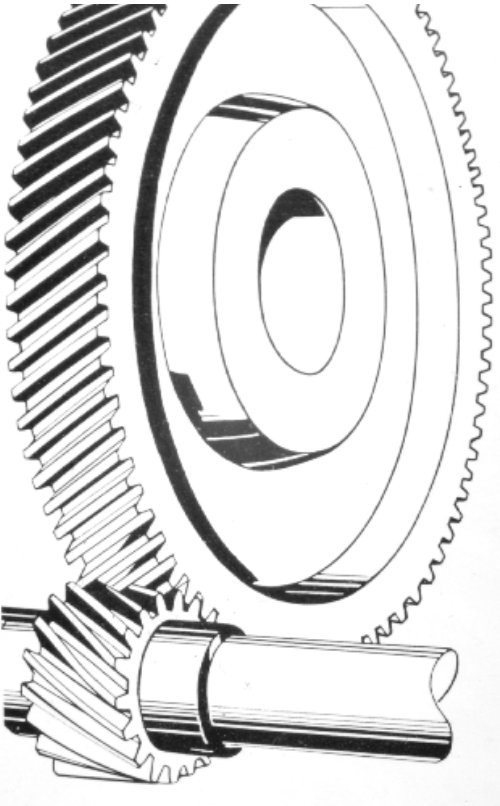
\includegraphics[scale=0.21]{ch1/9}
	\end{wrapfigure}	
	\noindent Pour remédier au problème de flexion, on réalise un engrènement progressif. Cependant, le problème des efforts radiaux laisse maintenant place aux efforts axiaux qui sont à l'origine de fatigue et d'usure sur les palier de guidage des arbres. Ce modèle est un peu plus compliqué mécaniquement. \\
	
\subsection{Engrenages cylindriques à chevrons}
	\begin{wrapfigure}[4]{r}{4cm}
	\vspace{-5mm}
	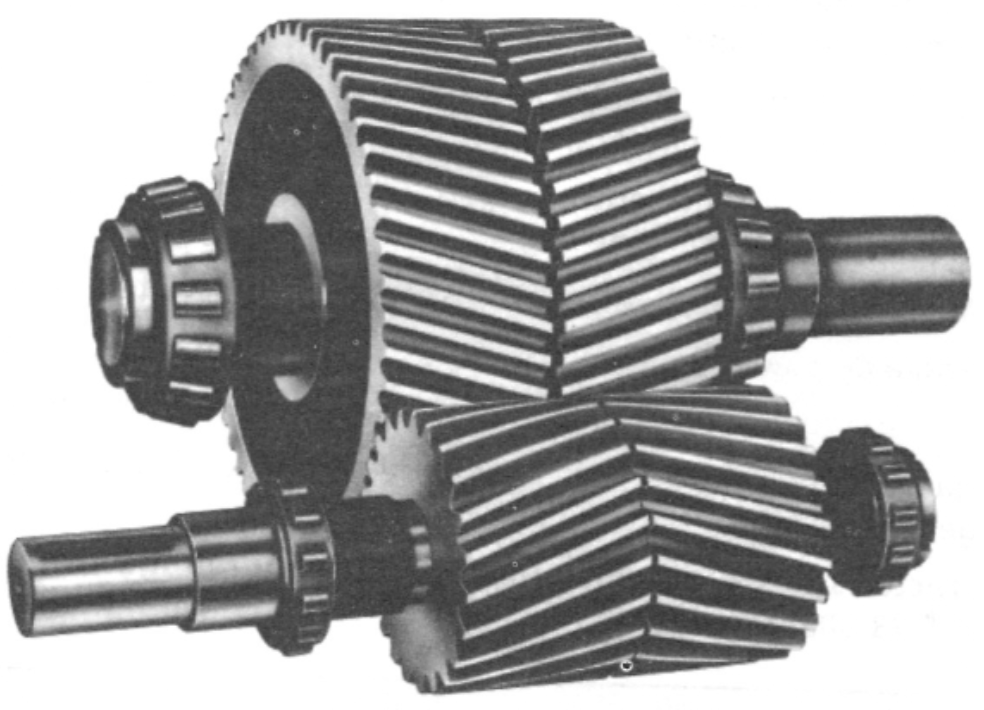
\includegraphics[scale=0.2]{ch1/10}
	\end{wrapfigure}	
	\noindent En utilisant des roues à chevrons, on espère, par effet opposé, d'annuler les contraintes axiales. Cependant, le coût de fabrication est élevé. \\
	
\subsection{Engrenages coniques}
	\begin{wrapfigure}[6]{l}{6.5cm}
	\vspace{-5mm}
	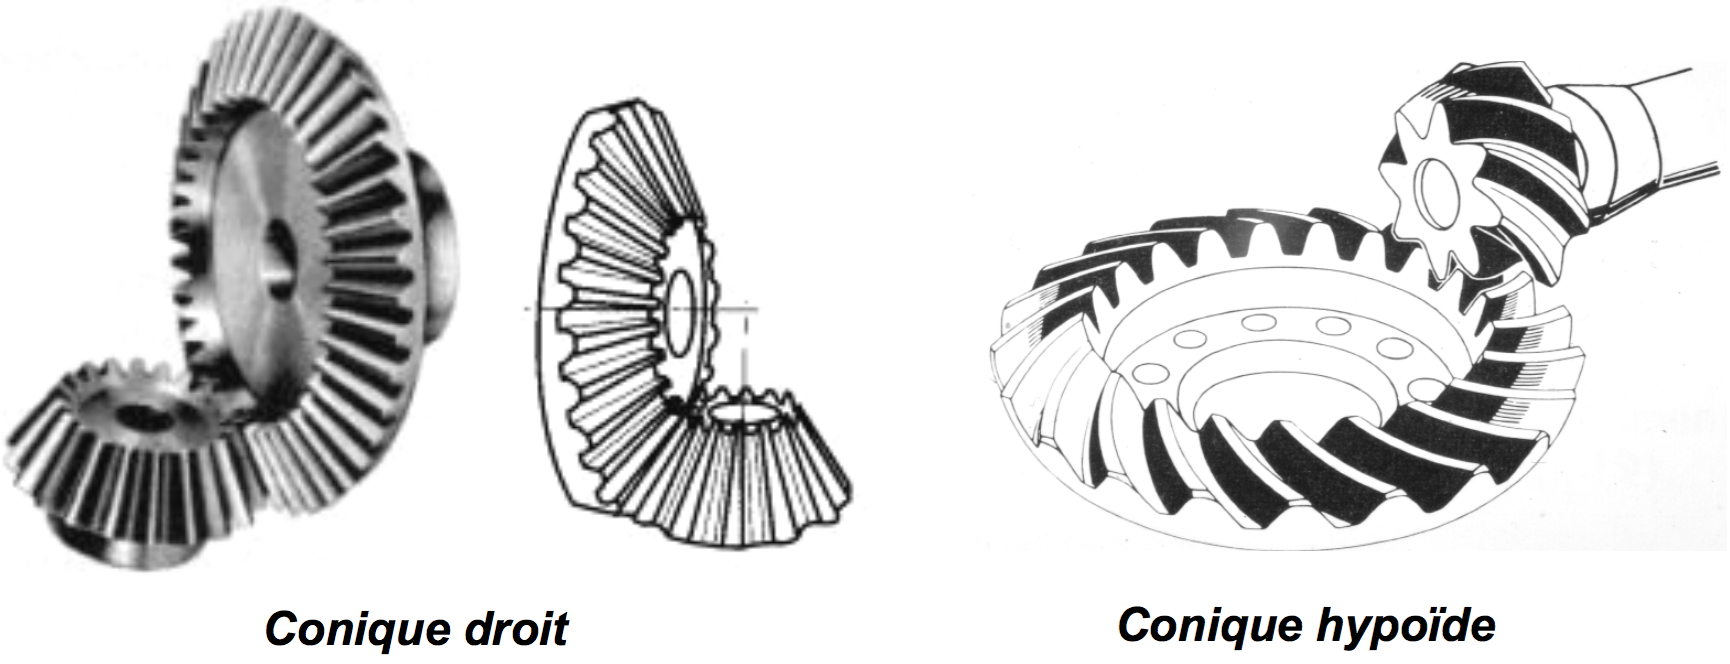
\includegraphics[scale=0.21]{ch1/11}
	\end{wrapfigure}	
	\noindent Ceux-ci sont utilisés lorsque les axes des engrenages ne sont pas parallèles. On distingue les \textbf{coniques droits} qui sont comparables aux dentures droites et les \textbf{hypoïdes} qui sont en fait les coniques hellicoïdales sauf que la développante de cercle est remplacée par une hypoïde.
	
\subsection{Engrenages gauches hellicoïdaux}
	\begin{wrapfigure}[2]{r}{4cm}
	\vspace{-5mm}
	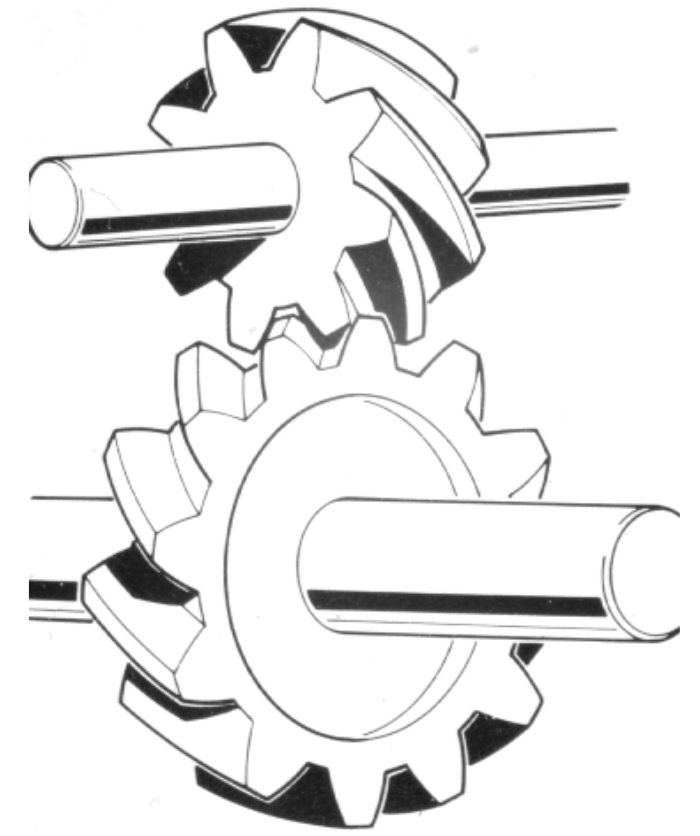
\includegraphics[scale=0.21]{ch1/12}
	\end{wrapfigure}	
	\noindent Là c'est l'extrême. Utilisé pour des axes quelconque. Très peu utilisé. \\\\\\\\

\subsection{Engrenages à roue et vis sans fin}
	\begin{wrapfigure}[6]{l}{2.5cm}
	\vspace{-5mm}
	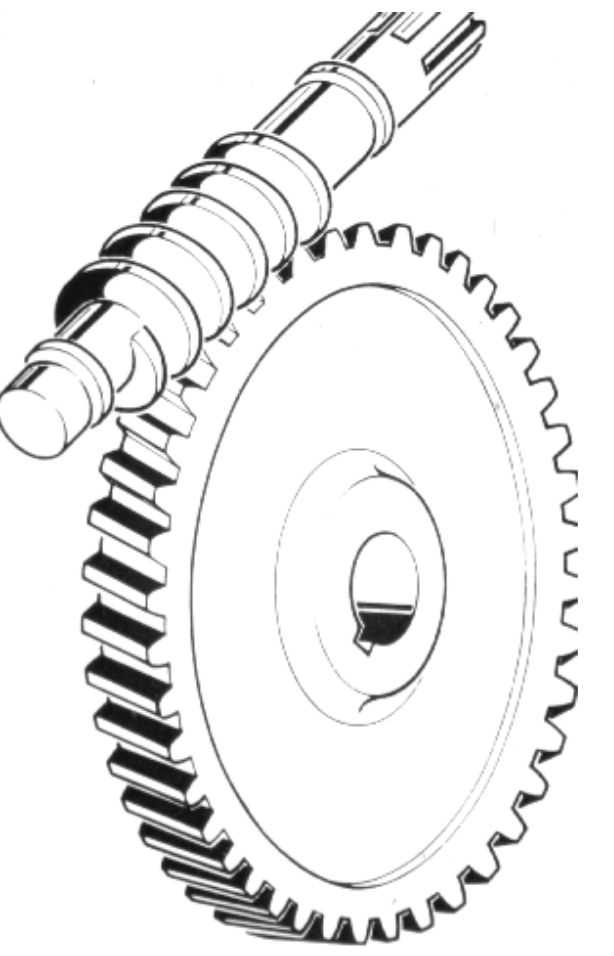
\includegraphics[scale=0.21]{ch1/13}
	\end{wrapfigure}	
	\noindent Ca ressemble à un pignon crémaillère en 3D qui ne translate pas, mais tourne. Il est intéressants pour le grand rapport de réduction ($\approx 1/200$). Cependant, le rendement est très faible et les glissements sont importants, causant de l'usure. Pour remédier à ce problème de glissement on peut utiliser une \textbf{roue creuse} (même modèle mais creusé. Pour concentrer l'usure sur la roue qui coûte moins cher, la vis est en acier et la roue en bronze (vis peut avoir plusieurs filets). \\
	
\section{Lubrification}
\noindent Pour une bonne lubrfication, il faut créer un \textbf{coin d'huile} qui permette de former une couche épaisse sous le solide en mouvement. Le gradient de pression permettra un meilleur glissement. La forme des dentures et le glissement au début du contact favorise la formation de ce coin d'huile. 

\subsection{Lubrification par barbotage}
	\begin{wrapfigure}[5]{r}{4cm}
	\vspace{-5mm}
	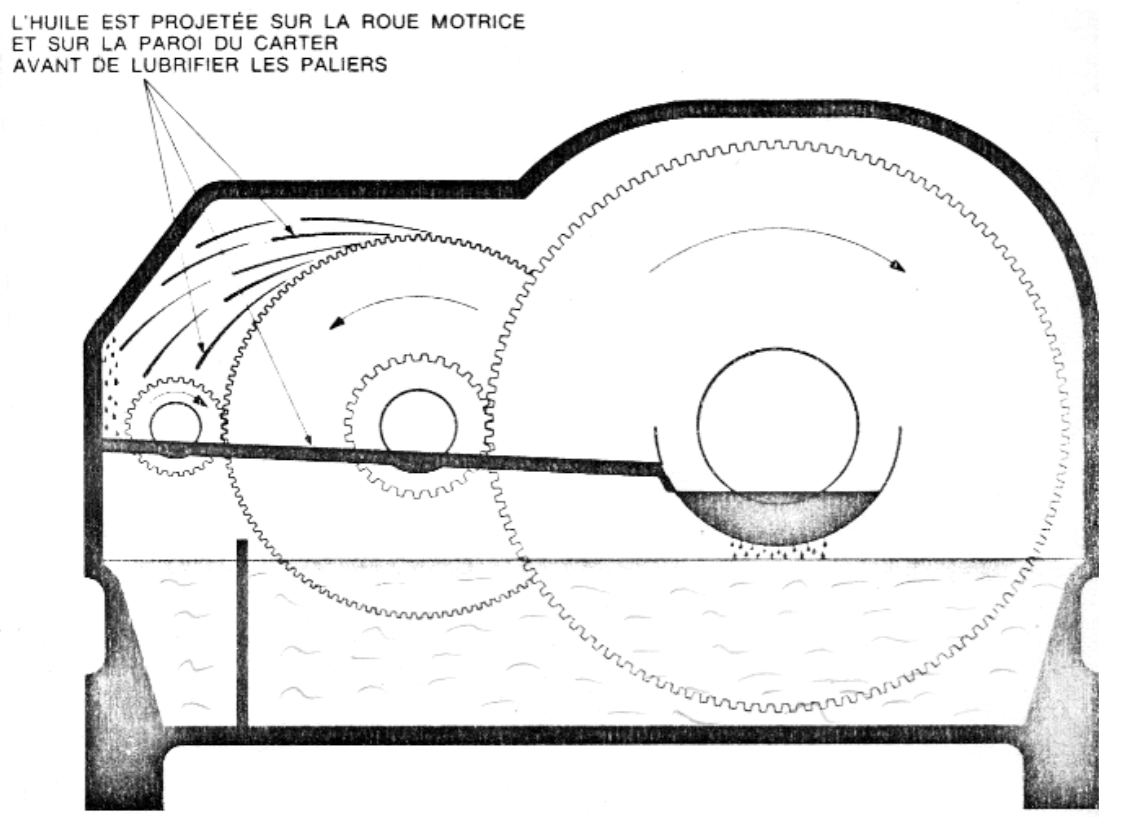
\includegraphics[scale=0.21]{ch1/14}
	\end{wrapfigure}	
	\noindent Il est débile de remplir toute la boîte d'huile en raison du coût, des frottements et du chauffage qui interviennent. On a un petit réservoir dans lequel les engrenages viennent tremper et projeter l'huile sur le mécnisme. Des \textbf{goutières} permettent de lubrifier les paliers. 
	
\subsection{Lubrification sous pression}
	\begin{wrapfigure}[6]{l}{4.5cm}
	\vspace{-5mm}
	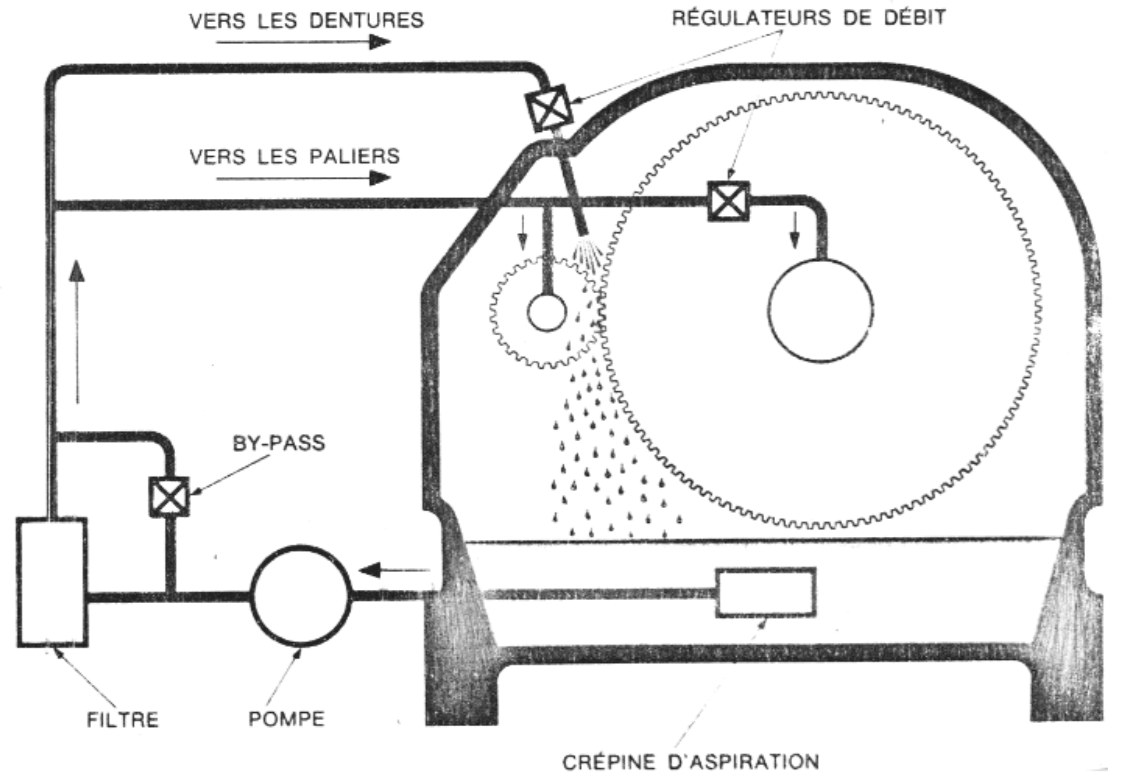
\includegraphics[scale=0.21]{ch1/15}
	\end{wrapfigure}	
	\noindent Ce mécanisme est utilisé pour de grosses puissances qui nécéssitent une lubrification dès le démarrage ainsi qu'un refroidissement important. Pour finir, dans le pire des cas, une lubrification par \textbf{graisse} peut protéger les pièces contre la corrosion, mais c'est sale. Notons que des pièces en \textbf{plastiques} sont également utilisées en raison de leur capacité auto-lubrifiante.